%%%%%%%%%%%%%%%%%%%%%%%%%%%%%%%%%%%%%%%%%
% Project Sky Net
% Design Dossier
% Version 1.0 (September 15, 2022)
%
% This template originates from:
% https://www.LaTeXTemplates.com
%
% Author:
% Braidan Duffy (bduffy2018@my.fit.edu)
% Subinita Dey (sdey2021@my.fit.edu)
% David Ephraim Vunnava (dvunnava@my.fit.edu)
%
% License:
% CC BY-NC-SA 4.0 (https://creativecommons.org/licenses/by-nc-sa/4.0/)
%
%%%%%%%%%%%%%%%%%%%%%%%%%%%%%%%%%%%%%%%%%

%----------------------------------------------------------------------------------------
%	CLASS, PACKAGES AND OTHER DOCUMENT CONFIGURATIONS
%----------------------------------------------------------------------------------------

\documentclass[
	letterpaper, % Paper size, use either a4paper or letterpaper
	12pt, % Default font size, the template is designed to look good at 12pt so it's best not to change this
	%unnumberedsections, % Uncomment for no section numbering
]{CSSullivanBusinessReport}

\addbibresource{sample.bib} % BibLaTeX bibliography file

\usepackage{longtable}

\usepackage{multirow}

\usepackage{xcolor}

\usepackage{colortbl}

\usepackage{pdflscape}

\usepackage{rotating}

\usepackage{amsmath}

%----------------------------------------------------------------------------------------
%	REPORT INFORMATION
%----------------------------------------------------------------------------------------

\reporttitle{Project Sky Net} % The report title to appear on the title page and page headers, do not create manual new lines here as this will carry over to page headers

\reportsubtitle{} % Report subtitle, include new lines if needed

\reportauthors{	Braidan Duffy (bduffy2018@my.fit.edu), \\
				Subinita Dey (sdey2021@my.fit.edu), \\
				David Ephraim Vunnava (dvunnava2022@my.fit.edu)} % Report authors/group/department, include new lines if needed

\reportdate{\today} % Report date, include new lines for additional information if needed

% \rightheadercontent{
\includegraphics[width=3cm]{creodocs_logo.pdf}} % The content in the right header, you may want to add your own company logo or use your company/department name or leave this command empty for no right header content

\setlength{\headheight}{3cm}
\fancyhead[C]{
    \begin{tabular}{ | p{8.5cm} | p{3cm} | p{3cm} | p{2.5cm} | }
        \hline
        Directorate of Advanced Development, PRN X-DHS20-013 & \multicolumn{3}{|c|}{Project Sky Net} \\
        \hline
         & \textbf{Revision:} & \textbf{Revision Date:} & \textbf{Page:} \\
        \hline
        Team: Futuristic Innovative Technologies (FIT) & 5 & \today & \thepage~of \pageref{LastPage} \\
        \hline
    \end{tabular}
}

%----------------------------------------------------------------------------------------

\begin{document}

%----------------------------------------------------------------------------------------
%	TITLE PAGE
%----------------------------------------------------------------------------------------

\thispagestyle{empty} % Suppress headers and footers on this page

\begin{fullwidth} % Use the whole page width
	\vspace*{-0.075\textheight} % Pull logo into the top margin
	
	% \hfill
\includegraphics[width=5cm]{creodocs_logo.pdf} % Company logo

	\vspace{0.15\textheight} % Vertical whitespace

	\parbox{0.9\fulltextwidth}{\fontsize{50pt}{52pt}\selectfont\raggedright\textbf{\reporttitle}\par} % Report title, intentionally at less than full width for nice wrapping. Adjust the width of the \parbox and the font size as needed for your title to look good.
	
	\vspace{0.03\textheight} % Vertical whitespace
	
	{\LARGE\textit{\textbf{\reportsubtitle}}\par} % Subtitle
	
	\vfill % Vertical whitespace
	
	{\normalsize\reportauthors\par} % Report authors, group or department
	
	\vfill\vfill\vfill % Vertical whitespace
	
	{\large\reportdate\par} % Report date
\end{fullwidth}

\newpage

%----------------------------------------------------------------------------------------
%	DISCLAIMER/COPYRIGHT PAGE
%----------------------------------------------------------------------------------------

\thispagestyle{empty} % Suppress headers and footers on this page

\begin{twothirdswidth} % Content in this environment to be at two-thirds of the whole page width
\footnotesize % Reduce font size

\subsection*{Disclaimer}

Lorem ipsum dolor sit amet, consectetur adipiscing elit. Praesent porttitor arcu luctus, imperdiet urna iaculis, mattis eros. Pellentesque iaculis odio vel nisl ullamcorper, nec faucibus ipsum molestie. Sed dictum nisl non aliquet porttitor. Etiam vulputate arcu dignissim, finibus sem et, viverra nisl. Aenean luctus congue massa, ut laoreet metus ornare in. Nunc fermentum nisi imperdiet lectus tincidunt vestibulum at ac elit.

\subsection*{Copyright}

\textcopyright~[2022] [Company] 

Copyright notice text\ldots In hac habitasse platea dictumst. Curabitur mattis elit sit amet justo luctus vestibulum. In hac habitasse platea dictumst. Pellentesque lobortis justo enim, a condimentum massa tempor eu. Ut quis nulla a quam pretium eleifend nec eu nisl. Nam cursus porttitor eros, sed luctus ligula convallis quis.

\subsection*{Contact}

150 W University Blvd\\
Department of Systems Engineering\\
Melbourne, FL 32901

Contact: sdey2021@my.fit.edu

\subsubsection*{Changelog}

\scriptsize % Reduce font size further

\begin{tabular}{@{} L{0.05\linewidth} L{0.15\linewidth} L{0.6\linewidth} @{}} % Column widths specified here, change as needed for your content
	\toprule
	v1.0 & 2022-09-15 & Initial document creation and editing\\
	\bottomrule
\end{tabular}
\end{twothirdswidth}

\newpage

%----------------------------------------------------------------------------------------
%	TABLE OF CONTENTS
%----------------------------------------------------------------------------------------

\begin{twothirdswidth} % Content in this environment to be at two-thirds of the whole page width
	\tableofcontents % Output the table of contents, automatically generated from the section commands used in the document
\end{twothirdswidth}

\newpage

%----------------------------------------------------------------------------------------
%	CONTENT
%----------------------------------------------------------------------------------------

\begin{fullwidth}
\section{Problem Statement}
    Futuristic Innovative Technologies (FIT) is a high-end producer of specialized UAV systems for extreme applications working to produce a feasibility study for building an Autonomous UAV (AUAV). This new AUAV would integrate state-of-the-art Atmospheric Turbulence Compensation (ATC) imaging capabilities with General Purpose Parallel Processing (GPPP) technology in real time, perform “search and find” maneuvers, track objects-of-interests, and avoid perceived threats. In addition to advanced optics that have ATC capability, the AUAV will have a hyperspectral and polarimetric imaging system on board that will be able to classify target composition from altitude. The AUAV must also be worldwide deployable, minimize or eliminate the use of sensitive electronics components, and have a neutral, nondescript profile.
    
    The AUAV will be controllable from a Mobile Command Center (MCC) that is capable of being powered off-grid for an indefinite amount of time in remote and low-access areas. The power requirements for the MCC are estimated to be 70-80 kWh and must utilize renewable energy resources as much as possible. The cabin of the MCC must also be human comfortable and able to give operators complete access to the AUAV command and control network as well as diagnostic and maintenance information. A component-level, bottom-up analysis of the MCC will also be performed in conjunction with the AUAV study.

\section{Mission Statement}
    The mission of the three-letter agency is to provide multi-purpose surveillance support for worldwide scientific collection activities, support low-profile data and information collection efforts for allies and national partners, conduct rapid worldwide deployments and surveillance activities in support of national treaty monitoring interests, and implement surveillance and reconnaissance missions for national strategic and tactical targets-of-interest (TOIs). The three-letter fosters science, innovative technology, and collaborations with strategic partners. 
    
\end{fullwidth}
\begin{fullwidth}
\section{Stakeholders}
\subsection{Point of Contact}
    The Point-of-Contact (POC) is Wilford Erasmus, Chief of Operations from the U.S. Department of Homeland Security and the U.S. Customs and Border Protection. The Chief of Operations is representing a 3-letter agency and is accountable for the project and customer interface. 

\subsection{The Customer}
    The Customer is a 3-letter agency represented by the U.S. Department of Homeland Security.

\subsection{Other Stakeholders}
    An investigation of other stakeholders yielded individuals and groups that Futuristic Innovative Technologies (FIT) may need to consult with, have negative interest in the project succeeding, or may benefit from the success of the project. Table \ref{tab:other_stakeholders} summarizes the other stakeholders for this project.
    \begin{longtable}{ | p{5cm} | p{12cm} | }
        \hline
        \rowcolor[gray]{.8}
        \textbf{Stakeholder Class} &  \textbf{Stakeholder Description} \\
        \hline
        External consultant & 
        \begin{itemize}
            \item Commercial Off The Shelf (COTS) suppliers
            \item Technical Subject Matter Experts (SME); if necessary
            \item Federal Aviation Administration (FAA)
            \item Federal Communications Commission (FCC)
            \item General Atomics - original developer of the AUAV
            \item National Weather Service (NWS)
            \item United States Embassies
            \item National Society of Professional Surveyors
            \item Air Force Research Laboratory (AFRL)
            \item Air Force Life Cycle Management Center (AFLCMC)
            \item Department of Transportation
        \end{itemize} \\
        \hline
        Negative stakeholders &
        \begin{itemize}
            \item Competitors (Northrup Grumman and other bidders)
            \item Civil liberty groups (e.g. American Civil Liberty Union)
            \item Citizen privacy groups (e.g. Electronic Privacy Information Center)
            \item Political parties (e.g. Democratic Party of America)
            \item Environmental and Ecological Organizations
        \end{itemize} \\
        \hline
        Functional Beneficiaries &
        Primary Stakeholders:
        \begin{itemize}
            \item 3-letter agencies
            \item International universities
            \item International research organizations
            \item International air and space agencies
            \item United States' allies and partners
            \item United States military
        \end{itemize} \\
         &
        Secondary Stakeholders:
        \begin{itemize}
            \item National Security Agencies (e.g. HSBP, FBI, CIA, ATF, DEA, DIA, US Marshals Service, local law enforcement, etc.)
            \item First responders (United States and international)
            \item United States Coast Guard
            \item National Park Service
            \item Aid organizations (e.g. USAID, Doctors Without Borders, etc.)
            \item Interpol
        \end{itemize} \\
        \hline
        \caption{Table of Other Stakeholders}
        \label{tab:other_stakeholders}
    \end{longtable}
    
    It is expected that the Federal Aviation Administration (FAA) will need to be consulted to obtain airframe and airworthiness certifications and that the State and Municipal Governments of the US. The Federal Communications Commission (FCC) will be consulted to obtain transmitting licenses. As well, FIT will need to consult with COTS suppliers for system components. Depending on the requirements, FIT may need to contract with, or sub-contract work to, subject matter experts (SMEs) to resolve deficiencies during the project.  General Atomics as the designer of the UAV being modified will need to be consulted for drawings, cable routing and other issues that will impact the design. Applicable Embassies will also need to be contacted to ensure proper permissions and certifications for overseas deployment.
    
    Although we believe that all design work can be performed in-house, FIT should be aware that Northrop Grumman and any other bidders are negative stakeholders that FIT may need to contract out for specialized components to adhere to schedule, cost, quality, and risk expectations are met, although direct competitors in the AUAV sector. The other negative stakeholders and functional beneficiaries will not be actively engaged in the project otherwise.
    
    Especially considering the benign appearance of the AUAV and the advanced search and rescue functions, the product may be of interest to agencies and organizations that regularly participate in rescue efforts in extreme environments. The product may be beneficial to these stakeholders with minimal changes or updates. 
    
    \subsection{The Hands-On Users}
    The project has identified five (5) entities that are the hands-on users. These are AUAV Flight Officers, AUAV Optical Operator, Intelligence Officers, AUAV Maintenance Technicians, and Mission Technicians

    Table \ref{tab:hands_on_users} shows each of the hands-on users’ current roles and responsibilities
    
    \begin{longtable}{ | p{5cm} | p{12cm} | }
        \hline
        \rowcolor[gray]{.8}
        \textbf{Stakeholder} & \textbf{Current Tasks} \\
        \hline
        AUAV Flight Officer &
        \begin{itemize}
            \item Remotely pilot the AUAV through taxiing, take-off, in-fight operations, and landing when the option for manual control is selected.
            \item Direct the AUAV to locations as ordered
            \item Update mission flight plans as ordered
            \item Select visibility mode (e.g. electro-optical during the day, Infrared radiation (IR) at night, or a combination at both in low-light times (e.g. dusk/dawn)
        \end{itemize} \\
        \hline
        AUAV Optical Operator &
        \begin{itemize}
            \item Orient electro-optical imaging on AUAV to view targets of interest
            \item Optimize and modify settings of AUAV during flight operations
            \item Monitor AUAV data streams and notify Flight Officer of situational anomalies
            \item Monitor AUAV status and direct to maintenance, as necessary
            \item Lock onto and track a target  while it remains stationary or move, relative to the AUAV
        \end{itemize} \\
        \hline
        Intelligence Officer &
        \begin{itemize}
            \item Interpret images from AUAV to confirm bipedal movement
            \item Initiate contact with land-based Mobile Command Centers (MCC)
            \item Confirm AI identification and detection of target
            \item Use obtained intelligence to guide AUAV operations and recommend course of action
            \item Verify operations are proceeding as planned
            \item Improvise new operational plan as situation and superiors dictate
        \end{itemize} \\
        \hline
        AUAV Maintenance Technicians &
        \begin{itemize}
            \item Perform pre and post-flight checkouts
            \item Fill fuel tanks, oil reservoirs, and other consumables
            \item Start and stop the AUAV engine
            \item Perform preventative maintenance, diagnostics, repairs, and servicing
            \item Help troubleshoot any mechanical failure during an operation
        \end{itemize} \\
        \hline
        Mission Technicians &
        \begin{itemize}
            \item Perform preventative maintenance, diagnostics, and repairs to the AUAV MCC, communication links, and associated systems
        \end{itemize} \\
        \hline
        \caption{Hands-On Users Current Roles and Responsibilities}
        \label{tab:hands_on_users}
    \end{longtable}
\end{fullwidth}
\begin{fullwidth}
\section{Stakeholders Needs and Requirements}

\end{fullwidth}
\begin{fullwidth}
\section{Concept of Operations}

\end{fullwidth}
\begin{fullwidth}
\section{Scope}
\subsection{scope statement}
The project's goals include integrating cutting-edge imaging capabilities in real time, performing "search and find" maneuvers, object of interest tracking.It is also designed to be extensible for future features and to account for the effects of atmospheric turbulence on imaging distortion and automatic target recognition. Additionally, FIT will conduct a feasibility assessment for the creation of a Mobile Command Center (MCC), which will be able to be permanently deployed in isolated, difficult-to-reach locations. The primary components of this project that must be internalized are:
\begin{itemize}
\item{Automatic Target Recognition (ATR) capability and high-speed atmospheric turbulence compensation(ATC).}

\item{The ability to track objects of interest (OoI) and conduct "search and locate" maneuvers, all autonomously.}

\item{provides advanced material and background discriminating capabilities with a polarimetric and hyperspectral imaging system.}

\item{The capacity to use a flexible system to augment other characteristics or capabilities based on the mission or environment in which it will be deployed.}
\end{itemize}
Features recommended for integration into AUAV must resemble generic 'Search and Rescue' characteristics for global deployment. The project's specific goal is to provide desert, coastline, and Alaskan wilderness search and rescue abilities, with an emphasis on adaptation to detect obstacles and resist itself owing to challenging conditions and circumstances. The system should be able to operate autonomously or be operated remotely.

\subsection{Scope Boundaries}
Below table categorizes the project tasks into 3 parts which are inter-related and integrated technologies.
\begin{table}
\centering
    \begin{tabular}{|p{5cm}| p{7cm}| p{2cm}|}
         \hline
          \rowcolor[gray]{0.8}
         System & Anticipated Task(s) & Exclusions\\[1ex]
         \hline
         Imaging capability with Atmospheric turbulence compensating system& \begin{itemize}
             \item {State-of-art technology}
             \item{Producing High spatial resolution images}
             \item{Environmental conditioning}
         \end{itemize}
         & None\\
        \hline
        Autonomous flight control system &
        \begin{itemize}
            \item{Object of interest tracking}
            \item{"Search and find" maneuvers}
            \item{Controllable manual over-ride}
            \item{Detect and identify target of Interest}
            \item{Controlled by a live operator}
        \end{itemize}
        & None\\
        \hline
        Adaptability&
        \begin{itemize}
            \item {Modular AUAV}
            \item{deploy-able World-wide, anytime of the day}
            \item{should be operable  even in extreme environment}
            \item{ability to be updated with newer hardware parts and software respectively}
            \item{disguised as a "search and rescue" AUAV}
        \end{itemize}
        & None\\
        \hline
    \end{tabular}
\end{table}
\end{fullwidth}
\begin{fullwidth}
\section{Goals and Objectives}
\subsection{Technical Goal(s)}
Within 16 weeks, a feasibility study of highly specialized features/capabilities for a potentially new AUAV for a three-letter national agency is to be completed. The customer has also requested baseline documentation and associated deliverables. Finally, the client has provided funding for FIT to do a feasibility study for a Mobile Command Center (MCC) that can be placed in a remote, difficult-to-access location. Table below outlines various tasks that must be completed as well as the estimated time for completion depending on the project commencement date.

 \begin{table}[!b]
    \centering
    \begin{tabular}{|p{5cm}|p{3cm}|p{7cm}|}
    \hline
    \rowcolor[gray]{0.8}
    Objective & Date of \newline Completion & Exit criteria\\
    \hline
    Initializing project & Week 0 & Project Award  \\
    \hline
    Problem Definition & Week 4\newline(+4 weeks) & Stakeholder's requirements are identified\\
    \hline
    Conceptual design Phase & Week 13\newline(+9 weeks) &
    A-spec documents are completed\\
    \hline 
    Preliminary design Phase & Week 15\newline(+2 weeks) & Preliminary Design Review completed\\
    \hline
    Final project & Week 16\newline(+1 weeks) & Proposal to three-letter agency complete\\
    \hline 
    \end{tabular}
\end{table}
\end{fullwidth}
\begin{fullwidth}
\section{Conceptual Design}
This section of the design dossier captures the system design associated with the conceptual design. Specifically, it defines the subsystem function block and functional flows that help add details to the System Specification.

Additional project risk analysis is provided in the form of a feasibility analysis on select requirements and the provided Failure Mode, Effect and Criticality Analysis.

\subsection{Functional Block Diagram}
    The focus of this project is to create a fleshed-out concept of an AUAV with a unique set of highly technical capabilities. This section will provide a high-level description of the functional systems within the AUAV. The aim is to show the overall relationships of the system. The  high-level functional block diagram, shown in Figure \ref{}, has been included to illustrate the various functions that make up the AUAV. In order to achieve a successful mission, all these functions must cooperate to achieve their objective while interacting with all of the other functions in the AUAV. 

    \begin{figure}
        \centering
        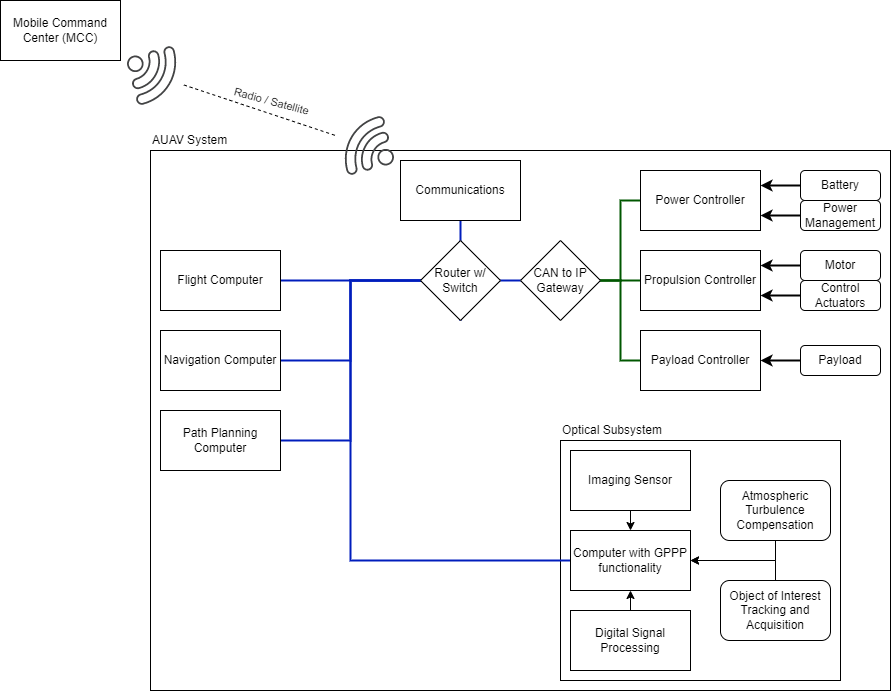
\includegraphics[height=6in]{01 - Design Dossier/images/UAV System Diagram-AUAV System.png}
        \caption{High Level System Functional Diagram}
        \label{fig:high_system_diagram}
    \end{figure}
\end{fullwidth}
\begin{fullwidth}
    \section{Analytic Hierarchy Process}
    The goal of the Analytic Hierarchy Process (AHP) is to determine an alternative from a given objective and set of criteria. This method is described in (Saaty, 2005) and allows alternatives to be relatively ranked to each other, providing the best alternative for the given criteria and objective. This study details two AHPs that were performed to determine the EO/IR sensor and the GPPP unit.

    The criteria and alternatives in an AHP analysis are ranked by the following metrics: \\
    \begin{table}[h!]
        \centering
        \begin{tabular}{|c|c|}
        \hline
            \textbf{Importance Scale} & \textbf{Definition of Importance of Scale} \\
            \hline
            1 & Equally important \\ \hline
            3 & Moderately important \\ \hline
            5 & Strongly important \\ \hline
            7 & Very strongly important \\ \hline
            9 & Extremely important \\
            \hline
        \end{tabular}
        \caption{Definition of importance in AHP analysis}
        \label{tab:ahp_importance_scale}
    \end{table}
    In the analysis, there can be intermediate values (i.e. 2, 4, etc.) that can be between the main values.

    \subsection{Electro-Optical/Infrared Sensor}
        For this analysis, three alternatives were chosen, as specified in Table \ref{tab:eoir_alternatives}. This analysis will compare each alternative with six criteria. The weightings of importance were provided by the stakeholders and FIT specialists

        \begin{table}[]
            \centering
            \begin{tabular}{|c|c|c|}
                \hline
                 \textbf{Alternative A} & \textbf{Alternative B} & \textbf{Alternative C} \\
                 \hline
                 \shortstack{High spatial \\ resolution sensor} & Multi spectral camera & Polarimetric Camera \\ \hline
            \end{tabular}
            \caption{Alternatives for the EO/IR detector}
            \label{tab:eoir_alternatives}
        \end{table}

        \newpage
        
        \begin{table}[h!]
            \centering
            \begin{tabular}{|c|c|c|c|c|c|c|}
                \hline
                 & \textbf{\shortstack{Maintenance \& \\ Support}} & \textbf{Reliability} & \textbf{\shortstack{Material \\ Discrimination}} & \textbf{Cost} & \textbf{\shortstack{Spatial \\ Resolution}} & \textbf{Weight} \\
                 \hline
                 \textbf{\shortstack{Maintenance \& \\ Support}} & $1$ & $\frac{1}{4}$ & $2$ & $\frac{1}{2}$ & $\frac{1}{3}$ & $2$ \\ \hline
                 \textbf{Reliability} & $4$ & $1$ & $8$ & $6$ & $4$ & $7$ \\ \hline
                 \textbf{\shortstack{Material \\ Discrimination}} & $\frac{1}{2}$ & $\frac{1}{8}$ & $1$ & $\frac{1}{4}$ & $\frac{1}{3}$ & $\frac{1}{2}$ \\ \hline
                 \textbf{Cost} & $2$ & $\frac{1}{6}$ & $4$ & $1$ & $\frac{1}{3}$ & $4$ \\ \hline
                 \textbf{\shortstack{Spatial \\ Resolution}} & $3$ & $\frac{1}{4}$ & $3$ & $3$ & $1$ & $2$ \\ \hline
                 \textbf{Weight} & $\frac{1}{2}$ & $\frac{1}{7}$ & $2$ & $\frac{1}{4}$ & $\frac{1}{2}$ & $1$ \\ \hline
            \end{tabular}
            \caption{EO/IR criteria preference matrix}
            \label{tab:eoir_preference_matrix}
        \end{table}

        When we find the Eigen vector of this matrix, we end up with the following priority vector:

        \[
        \left[ {\begin{array}{cc}
        0.090 \\
        0.478 \\
        0.044 \\
        0.142 \\
        0.183 \\
        0.063
        \end{array} } \right]
        \]

        There is a clear preference here for the reliability of the sensor, followed by the spatial resolution and cost. We can then compare each alternative with each other with respect to each criterion to get a consolidated alternative matrix shown below, where each row is an alternative and each column is a criterion:

        \[ 
        \left[ {\begin{array}{cccccc}
        0.537 & 0.620 & 0.198 & 0.633 & 0.286 & 0.297 \\
        0.195 & 0.156 & 0.312 & 0.261 & 0.143 & 0.164 \\
        0.268 & 0.224 & 0.491 & 0.106 & 0.571 & 0.539 \\
        \end{array} } \right]
        \]

        By multiplying the alternative matrix and the criterion priority matrices together, we can get a decision matrix shown in the table below. Here, we can see that Alternative A, the High spatial resolution camera is the best of the three proposed alternatives. The consistency ratio for this analysis is 0.068 which is below the 0.10 threshold indicating that this is a valid analysis.

        \begin{table}[]
            \centering
            \begin{tabular}{|c|c|c|}
                \hline
                \textbf{Alternative} & \textbf{Value} & \textbf{Rank} \\
                \hline
                A & 0.514 & 1 \\ \hline
                B & 0.179 & 3 \\ \hline
                C & 0.307 & 2 \\ \hline
            \end{tabular}
            \caption{Results from the AHP for the EO/IR sensor showing value and rank}
            \label{tab:eoir_ahp_results}
        \end{table}

    \subsection{General Purpose Parallel Processing Unit}
        The General Purpose Parallel Processing (GPPP) unit is a device that will perform the complex calculations on the EO/IR sensor's video feed to account for atmospheric turbulence and detect TOIs and OOIs. Six criteria were chosen and five alternatives analyzed. It was difficult to gather a consensus from the various stakeholders and FIT specialists on the weighting of the different criterion relative to each other. This introduces some error in the form of a high consistency ratio. However, the analysis is still believed to be valid.
    
        We can start by defining the five alternatives explored for this analysis as well as the six criteria.
    
        \begin{table}[h!]
                \centering
                \begin{tabular}{|c|c|c|c|c|c|}
                    \hline
                    \textbf{Criteria} & \textbf{Alternative A} & \textbf{Alternative B} & \textbf{Alternative C} & \textbf{Alternative D} & \textbf{Alternative E} \\
                    \hline
                    & \shortstack{Nvidia \\ RTX 4090} & \shortstack{Nvidia \\ RTX 3090 Ti} & \shortstack{Nvidia \\ RTX A100} & \shortstack{Nvidia \\ RTX A6000} & \shortstack{Nvidia \\ RTX A5000} \\ \hline
                    \textbf{\shortstack{FP32 \\ Performance}} & 83 & 40 & 20 & 39 & 28 \\ \hline
                    \textbf{\shortstack{Processor \\ Speed}} & 2235 & 1560 & 765 & 1410 & 1170 \\ \hline
                    \textbf{Cost} & \$1,600 & \$1,100 & \$10,000 & \$4,000 & \$2.500 \\ \hline
                    \textbf{\shortstack{Core \\ Count}} & 16384 & 10752 & 6912 & 10572 & 8192 \\ \hline
                    \textbf{\shortstack{Power \\ Consumption}} & 450 & 450 & 400 & 300 & 230 \\ \hline
                    \textbf{Memory} & 24 & 24 & 80 & 48 & 24 \\ \hline
                \end{tabular}
                \caption{Alternatives for the GPPP unit}
                \label{tab:gppp_alternatives}
        \end{table}

        Then, we can tabulate how the criteria compare with each other in terms of importance as rated by the stakeholders and specialists:

        \begin{table}[h!]
            \centering
            \begin{tabular}{|c|c|c|c|c|c|c|}
                \hline
                 & \textbf{\shortstack{FP32 \\ Performance}} & \textbf{\shortstack{Processor \\ Speed}} & \textbf{Cost} & \textbf{\shortstack{Core \\ Count}} & \textbf{\shortstack{Power \\ Consumption}} & \textbf{Memory} \\
                 \hline
                 \textbf{\shortstack{FP32 \\ Performance}} & $1$ & $\frac{1}{3}$ & $7$ & $\frac{1}{3}$ & $5$ & $1$ \\ \hline
                 \textbf{\shortstack{Processor \\ Speed}} & $3$ & $1$ & $5$ & $\frac{1}{3}$ & $3$ & $1$ \\ \hline
                 \textbf{Cost} & $\frac{1}{7}$ & $\frac{1}{5}$ & $1$ & $\frac{1}{5}$ & $3$ & $\frac{1}{5}$ \\ \hline
                 \textbf{\shortstack{Core \\ Count}} & $3$ & $3$ & $5$ & $1$ & $3$ & $1$ \\ \hline
                 \textbf{\shortstack{Power \\ Consumption}} & $\frac{1}{5}$ & $\frac{1}{3}$ & $\frac{1}{3}$ & $\frac{1}{3}$ & $1$ & $\frac{1}{7}$ \\ \hline
                 \textbf{Memory} & $1$ & $1$ & $5$ & $1$ & $7$ & $1$ \\ \hline
            \end{tabular}
            \caption{GPPP criteria preference matrix}
            \label{tab:gppp_preference_matrix}
        \end{table}

        The Eigen vector of this matrix gets us the following criteria priority vector:

        \[
        \left[ {\begin{array}{cc}
        0.169 \\
        0.212 \\
        0.053 \\
        0.304 \\
        0.044 \\
        0.218
        \end{array} } \right]
        \]

        Since their comparative weights are so relatively small to the other criteria, we can eliminate C3 (cost) and C5 (power) to reduce computational costs. When we perform the calculations to find the alternative priority vectors with respect to each criterion, we get the following matrix - again, each row is the alternative and each column is the criterion:

        \[ 
        \left[ {\begin{array}{cccccc}
        0.390 & 0.312 & 0.331 & 0.120 \\
        0.180 & 0.219 & 0.191 & 0.120 \\
        0.097 & 0.106 & 0.129 & 0.407 \\
        0.179 & 0.185 & 0.179 & 0.231 \\
        0.155 & 0.178 & 0.170 & 0.122 \\
        \end{array} } \right]
        \]

        When we multiply the two above matrices, we calculate the decision matrix shown below. Based off of this analysis, the project should proceed to use the Nvidia RTX 4090 as its GPPP unit followed by the RTX 3090 Ti and RTX A6000.

        \begin{table}[]
            \centering
            \begin{tabular}{|c|c|c|}
                \hline
                \textbf{Alternative} & \textbf{Value} & \textbf{Rank} \\
                \hline
                A & 0.238 & 1 \\ \hline
                B & 0.140 & 2 \\ \hline
                C & 0.096 & 5 \\ \hline
                C & 0.134 & 3 \\ \hline
                C & 0.121 & 4 \\ \hline
            \end{tabular}
            \caption{Results from the AHP for the GPPP unit showing value and rank}
            \label{tab:gppp_ahp_results}
        \end{table}        
\end{fullwidth}

%----------------------------------------------------------------------------------------
%	 REFERENCES/BIBLIOGRAPHY
%----------------------------------------------------------------------------------------

\newpage

\addcontentsline{toc}{section}{Reference List} % Add the bibliography to the table of contents

\begin{twothirdswidth} % Content in this environment to be at two-thirds of the whole page width
	\printbibliography[title=Reference List] % Output the bibliography with a custom section title
\end{twothirdswidth}

%----------------------------------------------------------------------------------------
%	APPENDICES
%----------------------------------------------------------------------------------------

\newpage

\section*{Appendices}

\begin{appendices}

\section{Project Terminology}
    \label{app:project_terms}
    \begin{longtable}{| p{6cm} | p{11cm} |}
        \hline
        \textbf{Project Terminology} & \textbf{Definition} \\
        \hline
        AIAA Standards & Engineering and technical requirements and the inclusion of provisions necessary to verify compliance \\
        \hline
        Airworthiness & Measure of an aircraft's suitability for safe flight \\
        \hline
        Atmosphere Turbulence & Small-scale, irregular air motions characterized by winds that vary in speed and direction \\
        \hline
        Automatic & A system that will do exactly as programmed; it has no choice \\
        \hline
        Autonomous & A system that can make a choice free from outside influence \\
        \hline
        Commercial Off The Shelf & Software and hardware that already exist and is available from commercial sources \\
        \hline
        dB & Decibel; measurement unit of sound \\
        \hline
        Electromagnetic Interference & Interference caused by one electrical or electric device to another by electromagnetic fields set up by its operation \\
        \hline
        Electromagnetic Radiation & Electric and magnetic disturbance traveling through space at the speed of light \\
        \hline
        Inertial Measurement Unit & A self-contained system that measures linear and angular motion using a triad of accelerometers and gyroscopes \\
        \hline
        MATLAB & An interactive programming environment for scientific computing \\
        \hline
        Mean Time Between Failure & Prediction of the time between failures of machinery pieces during normal operation parameters \\
        \hline
        Mean Time Between Repair & The average time it takes to repair a system; includes any repairs and testing time \\
        \hline
        Net Asset Value & Value of an entity’s assets minus the value of its liabilities, often in relation to open-end fund \\
        \hline
        Operational Availability & Measurement of the average availability over a period of time includes all experienced sources of downtime \\
        \hline
        Risk Priority Number & Measurement used when assessing risk to help, identify critical failure modes associated with design or process \\
        \hline
        Spatial Resolution & Measurement of the smallest object that can resolved by the sensor, or on the ground area image for the instantaneous field of view or the sensor \\
        \hline
        Subject Matter Expert & Individual or company has a deep understanding of a particular topic and can help improve products, solve problem, or meet technical challenges \\
        \hline
        Unmanned Aerial System & System whose components include the necessary equipment, networks, and personnel to control an unmanned aircraft \\
        \hline
        Unmanned Aerial Vehicle & Vehicle that does not carry a human operator and is capable of flight under remote control or autonomous programming \\
        \hline
        $(W/sr)$ & Watt per Steradian, SI unit of radiant intensity \\
        \hline
        $(W/m2)$ & Watt per Square Meter, SI unit of irradiate intensity\\
        \hline
    \caption{Project Terminologies}
    \label{tab:project_terms}
    \end{longtable}

\end{appendices}

%----------------------------------------------------------------------------------------

\end{document}
